\documentclass{ieeeaccess}
\usepackage{cite}
\usepackage{amsmath,amssymb,amsfonts}
\usepackage{algorithmic}
\usepackage{graphicx}
\usepackage{textcomp}
\usepackage{listings}
\def\BibTeX{{\rm B\kern-.05em{\sc i\kern-.025em b}\kern-.08em
    T\kern-.1667em\lower.7ex\hbox{E}\kern-.125emX}}
\begin{document}

\doi{11.4514/ACCESS.2024.1919810}

\title{Preparation of Papers for IEEE ACCESS}

\author{XIAN Chong\authorrefmark{1}, ZHANG
    Kaidi\authorrefmark{2}, ZENG Junqi\authorrefmark{3}, LIN Fanyue\authorrefmark{4}, and YU Shijiong\authorrefmark{5}}

\address[1]{22097486D}
\address[2]{22100265D}
\address[3]{22099611D}
\address[4]{22099314D}
\address[5]{22107027D}

\begin{abstract}
This project aims to create an application for a medium-sized steel manufacturer to better arrange the production schedules of its three factories (Factory X, Y, and Z) and improve the utilization of the factories. The main algorithms are First Come First Serve (FCFS) and Priority (PR). The development of this application will help improve the company's production efficiency and profit margin.
\end{abstract}

\titlepgskip=-21pt

\maketitle

\section{Introduction}
\label{sec:introduction}
\PARstart{T}{his} article presents PLS, an application designed to optimize production scheduling for medium-sized steel manufacturers. The company operates three factories, but due to ineffective production planning, factory efficiency is low, resulting in delayed orders and decreased profits. The application's main objective is to enhance the production capacity of the three factories and determine which orders to accept or reject. Accepting an order that cannot be completed on time will result in profit losses. The application aims to improve the company's production efficiency and profit margin.

\subsection{Related work}
A few related concept is use by the program.

Firstly, interrupts and system calls. A system call is a programming interface to the services provided by the OS. System call is widely used in the program, and it is the foundation of the programming process in this project. W ehis program use interrupts when errors occur.

Secondly, file management. This knowledge is also significant in the project, as it are mainly processing several files, the input and output.

Thirdly, scheduling algorithms. Process scheduling is the activity of deciding which process should be performed first (or when), based on a particular strategy/algorithm. This activity is performed by the process manager; as it removes an active process from the CPU and selects another from the queue. The need for scheduling in OS arises since most applications are multi-programing, i.e. they allow for multiple processes to be loaded and shared with the CPU at a point in time. The manager needs to make the decision on which of these processes must be performed first. We chose First Come First Serve (FCFS) and Priority (PR) as our algorithms when scheduling processes given to factories.

We might have covered some other topics with small relationships, for example process management, memory management and so on.

\subsection{Concept}
This project implements the three scheduling algorithms, including FCFS and PR.

In FCFS, processes are served in their arrival order. This algorithm can maintain the fairness of each coming process(order). Processes may arrive around the same time. Often the process pid could reflect the real arrival order, since the earlier process would normally receive a smaller pid. By this characteristic, FCFS algorithm is implemented.

In PR, a priority number is associated with each process. CPU is allocated to the process with highest priority. In some systems, largest value in priority means highest priority (Windows), and in some others, smallest value means highest priority (Unix and Linux). Again, priority scheduling could be either non-preemptive or preemptive. Although the preemptive version is more commonly in use, it is possible that process with higher priority level may arrive in a short time after starting processing one order, and it is not so functional when we pause the current processing order and choose to finish the new one. So, this program will only put the new process in the waiting line. If a lot of orders are given in a short time, the program will divide them into different priority levels and then use FCFS algorithm to make further distribution.

\subsection{Critical Deadline First scheduling algorithm}
The Critical Deadline First (CDF) scheduling algorithm operates by prioritizing tasks based on their respective deadlines. When executing the CDF algorithm, tasks with closer deadlines are given higher priority, ensuring that time-sensitive activities are completed promptly. By focusing on meeting critical due dates, the CDF algorithm optimizes task scheduling and resource allocation. This approach minimizes the risk of missing important deadlines and helps maintain a high level of efficiency in time-constrained environments. Through the careful arrangement of tasks according to their deadlines, the CDF algorithm facilitates effective task management and ensures timely completion of critical activities.

\section{Methodology}

\subsection{Software structure}
The software structure of the system is designed to ensure effective organization and management of its various components. The source code, located in the \texttt{src} directory, is divided into four parts: input, output, runpls, and tools, each has corresponding .h and .c files. The input part handles reading input format, while the output part is responsible for analyzing and output data. The runpls part executes the scheduling algorithm, which results will be sent to the output component. The tools part provides supplementary functionalities and utilities for this project. Additionally, a main.c file serves as the system's entry point. The \texttt{build} directory contains the necessary files for building the system, including a makefile, temporary object files, and the final executable. The \texttt{report} directory houses the system's report, comprising the tex source code and a PDF version. Additionally, there are auxiliary files such as \texttt{.gitignore} to exclude specific files from version control, \texttt{README.md} to offer an introduction and basic information about the system in a more readable way, \texttt{LICENSE} to declare the licensing terms, and the \texttt{.git} directory to store Git-related information. This software architecture allows for efficient development, building, reporting, and version control processes, maintaining the system's integrity and ease of maintenance.

\subsection{Testing}
\subsubsection{Testing Method}
First, a large number of random and different \texttt{addORDER} command is genrated via datagen program and these orders are sent into the system after creating the \texttt{addPERIOD}. Subsequently, the algorithm run section is executed, allowing each algorithm to execute the order allocation procedure separately and ouput it. By double-checking that the orders in the report are in the right place, the program is allocating the orders accurately as expected.

\subsubsection{Performance analysis}
In our study about production scheduling, It is wanted to understand which algorithms were best at making the most of the resources and getting things done quickly.30 tests were ran to carefully test three main algorithms: Priority Rules (PR), Critical Duedate First (CDF), and First Come First Served (FCFS). How well each algorithm used our resources on average is the main concern in this project.

The one of results we got gave us some interesting insights into how these scheduling methods compare. Each algorithm showed its own strengths and weaknesses throughout our tests.

\textbf{First Come First Served (FCFS)}: FCFS, though a basic method, didn't use the resources as efficiently, with only a 71\% average utilization rate.

\textbf{Priority Rules (PR)}: PR managed to use about 75.3\% of our resources on average. This algorithm decides which tasks are most important based on certain rules, like when they are due or what kind of product they are. By ordering tasks strategically, PR aims to make sure the program use the resources well and keep production running smoothly.

\textbf{Critical Duedate First (CDF)}: CDF turned out to be the best performer out of the three, with an average resource utilization of 84.3\%.

\section{Program set up and execution}
This project should be set up and execution in apollo mechaine. Some other environment in linux might be support but not guranted. This program requires nothing but the C standard library. To setup the program, navigate to the buildory directory, which is \texttt{./build}. Once in the build directory, the system is built by running the \texttt{make} command in bash, resulting in the creation of the executable file named \texttt{PLS} within the build directory. To execute the system, one must first enter the build directory using the \texttt{cd build} command. Subsequently, the system is launched by running the \texttt{./PLS} command. Upon execution, the user is prompted to input a command. Several command options are available, including \texttt{addPERIOD} for specifying start and end dates, \texttt{addORDER} for providing order details such as order number, due date, quantity, and product name, \texttt{addBATCH} for processing orders from a batch file, \texttt{runPLS} for executing a specific algorithm and generating a report file, and \texttt{exitPLS} for terminating the system. It is important that the \texttt{addPERIOD} command should be the first command when excluding, and the batch file for \texttt{addBATCH} should only include the \texttt{addORDER} command. When using commands that require a file, the user could provide the relative path of the file. To try one test data, the \texttt{datagen.sh} might be used by \texttt{./datagen.sh > inputBatch.dat}. By following these steps, the program can be set up and executed effectively, enabling the user to interact with the system and perform various operations as required.

\section{Results}
The scheduling program yielded significant results in optimizing task assignments. Fig. \ref{FCFS} illustrates the outcome of employing the First-Come-First-Serve (FCFS) scheduling algorithm, showcasing improved task completion times. Fig \ref{PR} presents the results obtained through the Critical Deadline First (CDF) algorithm, demonstrating enhanced prioritization of time-sensitive tasks. Finally, Fig. \ref{CDF} presents the output of the Priority (PR) algorithm, highlighting the efficiency achieved through task prioritization. For a comprehensive overview of the complete results, please refer to the appendices.

\begin{figure}[h]
    \centering
    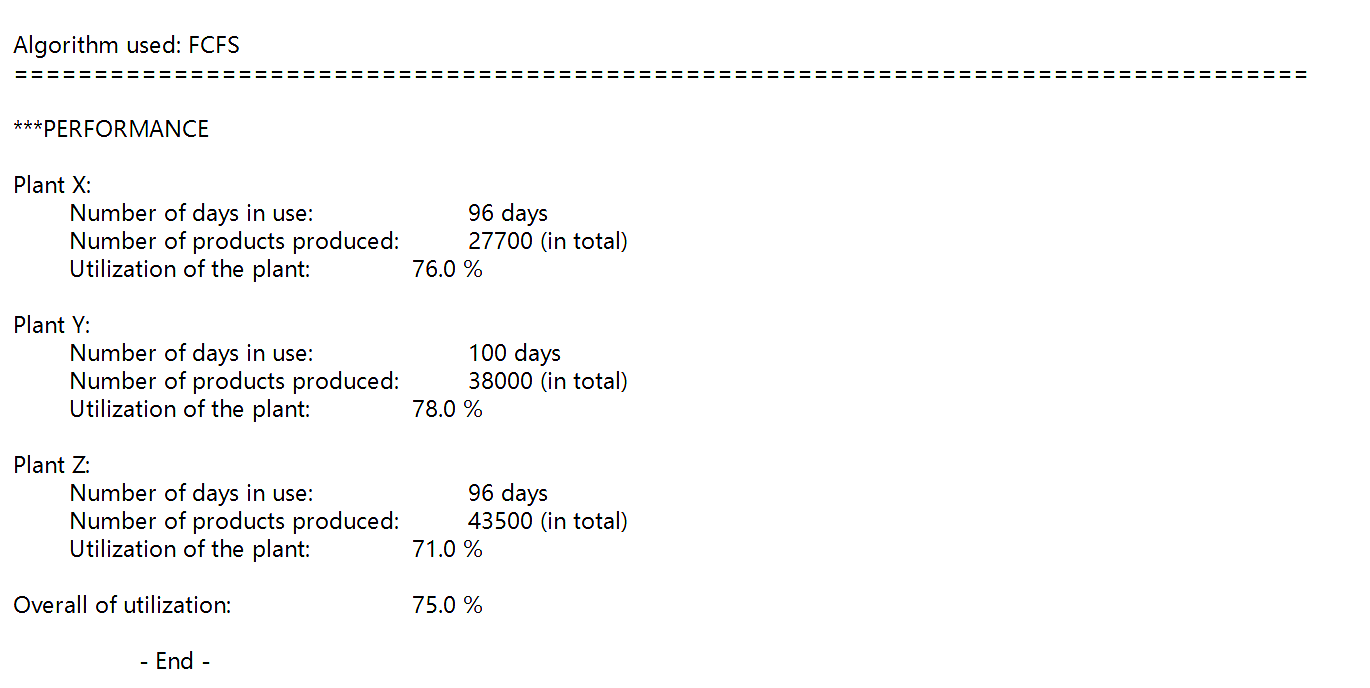
\includegraphics[width=88mm]{image/1.png}
    \caption{The result of the FCFS algorithm.}
    \label{FCFS}
\end{figure}

\begin{figure}[h]
    \centering
    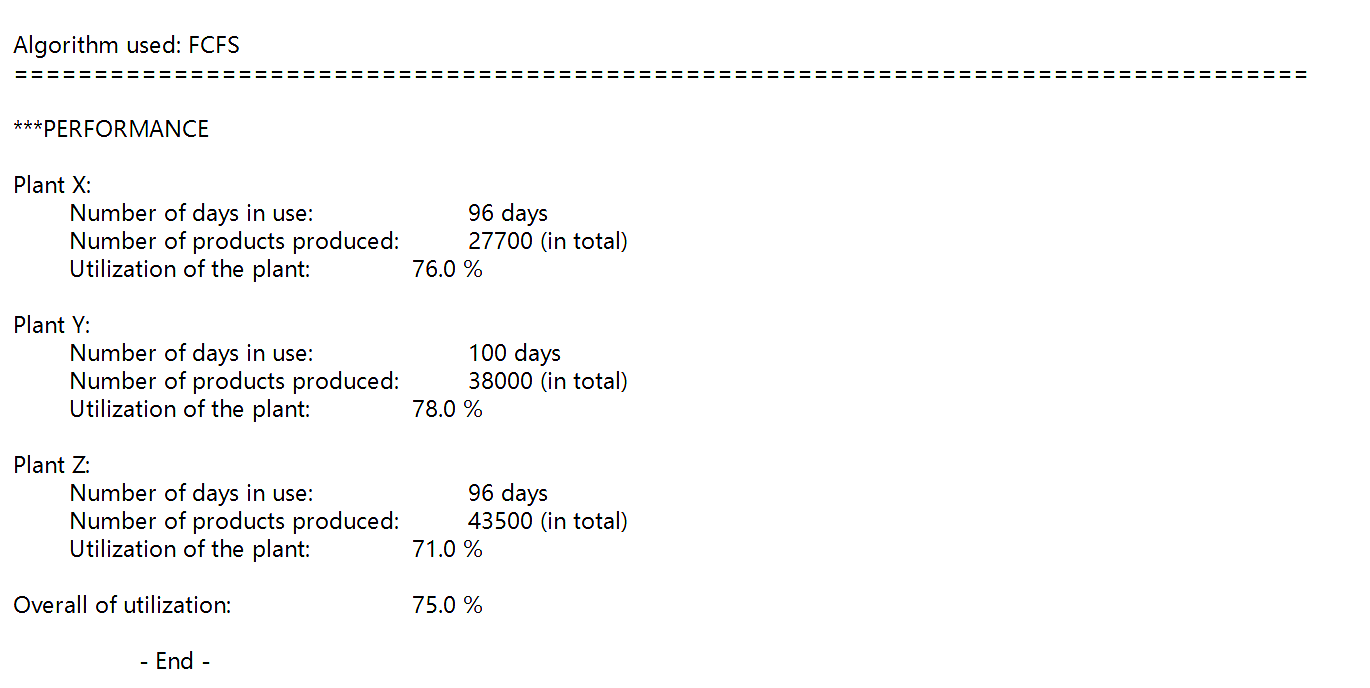
\includegraphics[width=88mm]{image/1.png}
    \caption{The result of the PR algorithm.}
    \label{PR}
\end{figure}

\begin{figure}[h]
    \centering
    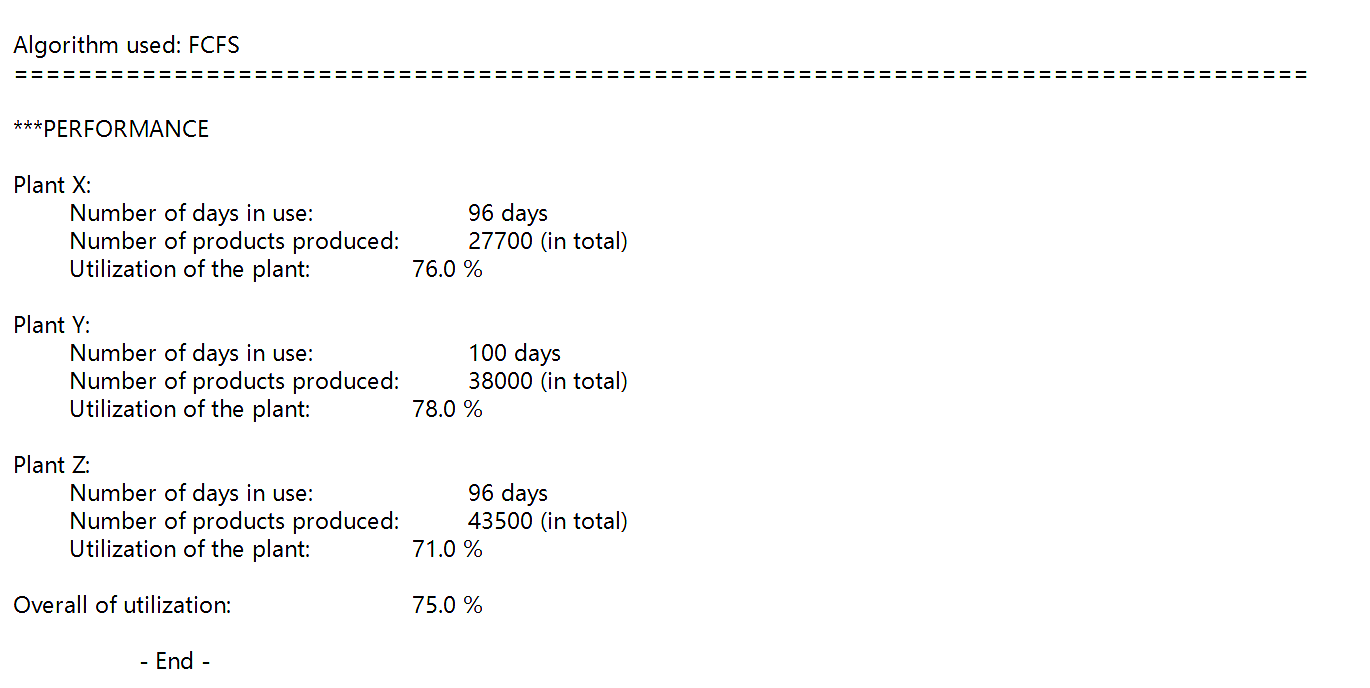
\includegraphics[width=88mm]{image/1.png}
    \caption{The result of the CDF algorithm.}
    \label{CDF}
\end{figure}

\section{Conclusion}
This project aims to develop an application for a medium-sized steel manufacturer to improve the scheduling of production plans for its three factories (Factory X, Y, and Z) and enhance factory utilization. The main algorithms used are First Come First Served (FCFS) and Priority (PR). The implementation of this application will significantly enhance the company's production efficiency and profit margin.


\appendices
\section{\break source code file}
\lstset{literate={=}{{=\allowbreak}}{1}}
\subsection{input.c}
\lstinputlisting[language=c, breaklines=true]{../../src/input.c}
\subsection{input.h}
\lstinputlisting[language=c, breaklines=true]{../../src/input.h}
\subsection{main.c}
\lstinputlisting[language=c, breaklines=true]{../../src/main.c}
\subsection{output.h}
\lstinputlisting[language=c, breaklines=true]{../../src/output.h}
\subsection{output.c}
\lstinputlisting[language=c, breaklines=true]{../../src/output.c}
\subsection{runpls.c}
\lstinputlisting[language=c, breaklines=true]{../../src/runpls.c}
\subsection{runpls.h}
\lstinputlisting[language=c, breaklines=true]{../../src/runpls.h}
\subsection{tools.c}
\lstinputlisting[language=c, breaklines=true]{../../src/tools.c}
\subsection{tools.h}
\lstinputlisting[language=c, breaklines=true]{../../src/tools.h}

\section{\break sample outputs}

\subsection{report\_CDF.txt}
\lstinputlisting[breaklines=true]{../../build/report_CDF.txt}
\subsection{report\_FCFS.txt}
\lstinputlisting[breaklines=true]{../../build/report_FCFS.txt}
\subsection{report\_PR.txt}
\lstinputlisting[breaklines=true]{../../build/report_FCFS.txt}

\EOD

\end{document}

%%% Local Variables:
%%% mode: LaTeX
%%% TeX-master: t
%%% End:
